% Created 2021-10-06 mar 13:05
% Intended LaTeX compiler: pdflatex
%%% Local Variables:
%%% LaTeX-command: "pdflatex --shell-escape"
%%% End:
\documentclass[11pt]{article}
\usepackage[utf8]{inputenc}
\usepackage[T1]{fontenc}
\usepackage{graphicx}
\usepackage{grffile}
\usepackage{longtable}
\usepackage{wrapfig}
\usepackage{rotating}
\usepackage[normalem]{ulem}
\usepackage{amsmath}
\usepackage{textcomp}
\usepackage{amssymb}
\usepackage{listings}
\usepackage{capt-of}
\usepackage{hyperref}
\hypersetup{colorlinks=true, linkcolor=black}
\setlength{\parindent}{0in}
\usepackage[margin=1.1in]{geometry}
\usepackage[spanish]{babel}
\usepackage{mathtools}
\usepackage{palatino}
\usepackage{fancyhdr}
\usepackage{sectsty}
\usepackage{engord}
\usepackage{cite}
\usepackage{graphicx}
\usepackage{setspace}
\usepackage[compact]{titlesec}
\usepackage[center]{caption}
\usepackage{placeins}
\usepackage{tikz}
\usetikzlibrary{positioning}
\usetikzlibrary{bayesnet}
\usetikzlibrary{shapes.geometric}
\usetikzlibrary{decorations.text}
\usepackage{color}
\usepackage{amsmath}
\usepackage{minted}
\usepackage{pdfpages}

\def\inline{\lstinline[basicstyle=\ttfamily,keywordstyle={}]}

\titlespacing*{\subsection}{0pt}{5.5ex}{3.3ex}
\titlespacing*{\section}{0pt}{5.5ex}{1ex}
\author{José Antonio Álvarez Ocete\\ Francisco Javier Sáez Maldonado}
\date{\today}
\title{Introducción a Hadoop y Spark\\\medskip
\large Procesamiento de Datos a Gran Escala}
\begin{document}

\maketitle

\tableofcontents

\section{Parte 1}

\subsection{Proceso}

Instalamos Java


\begin{minted}{bash}
yum install java-1.8.0-openjdk-devel
\end{minted}

Cambiamos la versión por defecto que se usaba en las transparencias. Incluso si instalamos la versión 1.7 se instalará la versión 1.8. Hemos de cambiar los paths a las versión 1.8 para que funciona correctamente:
\begin{minted}{bash}
export JAVA_HOME=/usr/lib/jvm/jre-1.8.0-openjdk
\end{minted}

Editamos el archivo  \inline{/opt/hadoop/etc/hadoop/hadoop.env.sh}:
\begin{minted}{bash}
export JAVA_HOME=/usr/lib/jvm/jre-1.8.0-openjdk
\end{minted}



\subsubsection*{ Compilación}

Tomamos el código que se ha proporcionado y lo compilamos utilizando la orden

\begin{minted}{bash}
bin/hadoop fs -cat /user/bigdata/compilar.bash | exec bash -s WordCount
\end{minted}

\subsubsection*{ Ejecución }

Primero hay que iniciar el NameNode y el DataNode:
\begin{minted}{bash}
sbin/start-dfs.sh
\end{minted}

Iniciar el ResourceManager y el NodeManager:

\begin{minted}{bash}
sbin/start-yarn.sh
\end{minted}

Recuerda que hemos de subir el archivo utilizando:
\begin{minted}{bash}
/opt/hadoop/bin/hdfs dfs -put Quijote.txt /user/root
\end{minted}

Lanzamos nuestro trabajo de MapReduce:

\begin{minted}{bash}
sudo /opt/hadoop/bin/hadoop jar WordCount.jar uam.WordCount Quijote.txt output/
\end{minted}

Obtenemos en el directorio output la salida. En concreto, dos archivos:
\begin{itemize}
\item Un archivo  \inline{SUCCESS }indicando que la tarea ha sido exitosa.
\item Un archivo  \inline{part-r-00000 }que tiene la salida del programa que queríamos ejecutar.
\end{itemize}

Mostramos una parte del fichero para mostrar parte de la salida.

\begin{minted}{bash}
    "Tablante",	1
    "dichosa	1
    "el	8
    "y	1
    (Y	1
    (a	1
    (al	1
    (como	1
    (creyendo	1
    (de	2
    (por	2
    (porque	2
    (pues	1
    (que	21
\end{minted}

Como podemos comprobar, las palabras quedan con ciertos símbolos de puntuación que no nos interesa que estén para realizar el conteo correcto de palabras. 

\subsubsection*{ Modificación del programa }

Para arreglar esto, solo debemos cambiar una linea en la función \inline{Map }del archivo  \inline{WordCount.java}. En concreto, la dejamos de la siguiente forma:

\begin{minted}{java}
StringTokenizer itr = new StringTokenizer(value.toString().
        toLowerCase().replaceAll("[^a-z ]", ""));
\end{minted}
como vemos, hemos pasado las palabras a minúsculas usando \inline{toLowerCase }y luego hemos eliminado todo aquello que no sean letras usando  \inline{replaceAll}.

Una vez realizada esta modificación, debemos compilar de nuevo el programa como lo hemos hecho anteriormente y, seguidamente, ejecutar de nuevo el programa java para que realice el conteo de palabras. En este caso, indicamos que la salida la realice sobre la carpeta  \inline{output2/} para tener las dos salidas por separado y poder compararlas. Obtenemos los dos mismos ficheros que anteriormente.

Hecho esto, utilizamos el archivo  \inline{script.py} que hemos creado usando  \inline{Python}, que toma todas las palabras que hay en los ficheros de salida y el número de veces que aparece cada una, las ordena y toma las 10 primeras para mostrarlas por pantalla. 

El resultado que se obtiene es que las palabras son las mismas y prácticamente en el mismo orden, salvo una pequeña variación entre dos de ellas. Podemos verlo gráficamente en la siguiente figura:

\begin{figure}[H]
\centering
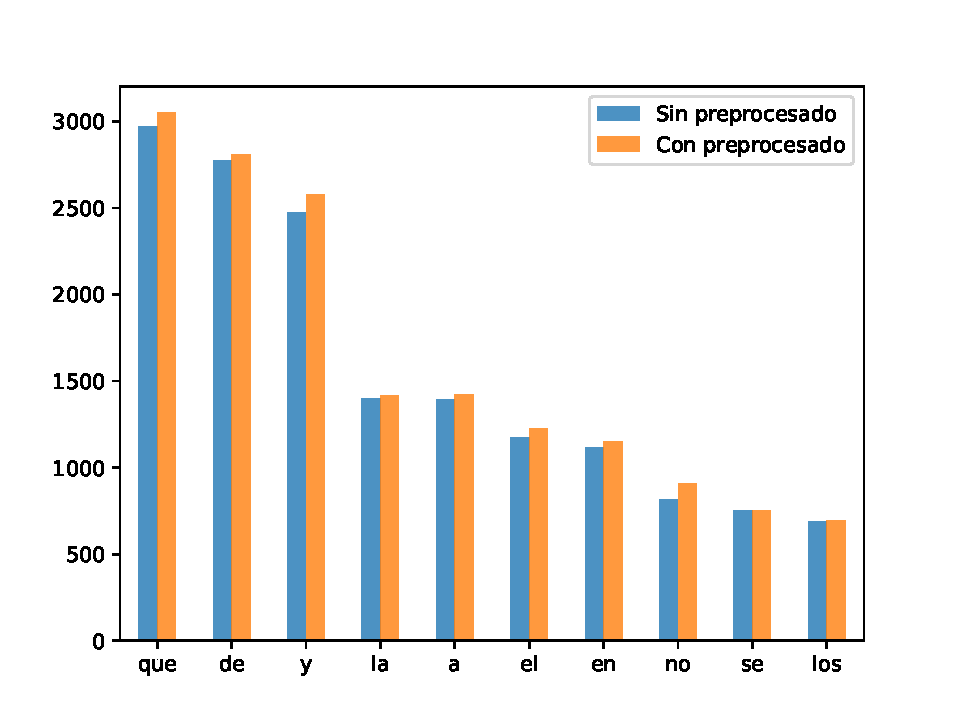
\includegraphics[scale=0.8]{barplot.pdf}
\caption{Comparación de número de veces que aparece cada palabra con y sin preprocesamiento.}
\end{figure}

Se puede apreciar que, al aplicar el preprocesado, la palabra \inline{a }aparece un número de veces ligeramente superior al que lo hace cuando no tenemos el preprocesador previo del texto.


\subsubsection*{ Comparación de resultados con otros ejemplos}

TODO







\subsection{ Cuestiones planteadas}

\subsubsection*{ Pregunta 1.1. ¿ Qué ficheros ha modificado para activar la configuración del HDFS? ¿ Qué líneas ha sido necesario modificar?}

Hemos modificado el fichero \inline{/opt/hadoop-2.8.1/etc/hadoop/hadoop-env.sh }añadiendo la línea \inline{export JAVA_HOME= /usr/lib/jvm/jre-1.7.0-openjdk }para especificar la instalación de \inline{Java }que queremos utilizar.


Como se explica en  \href{https://stackoverflow.com/questions/17569423/what-is-best-way-to-start-and-stop-hadoop-ecosystem-with-command-line}{esta respuesta de Stack Overflow}, el script \inline{stop-all.sh }detiene todos los daemons de Hadoop a la vez, pero está obsoleto. En lugar de eso es recomendable parar los daemons de HDFS y YARN por separado en todas las máquinas utilizando \inline|stop-dfs.sh| y  \inline{stop-yarn.sh}.

A continuación, para instalar Hadoop pseudo-distribuido, hemos modificado el fichero 
\begin{minted}{bash} 
    /opt/hadoop/etc/hadoop/core-site.xml
\end{minted}
del siguiente modo:


\begin{minted}{xml}
<configuration>
    <property>
        <name>fs.defaultFS</name>
        <value>hdfs://localhost:9000</value>
    </property>
</configuration>
\end{minted}


Y añadimos al fichero  \inline{/opt/hadoop/etc/hadoop/hdfs-site.xml} lo siguiente:
\begin{minted}{xml}
<configuration>
    <property>
        <name>dfs.replication</name>
        <value>1</value>
    </property>
</configuration>
\end{minted}

A continuación, hemos realizado la instalación del sistema pseudo-distribuido usando  \inline{YARN}, así que hemos modificado los siguientes ficheros \textbf{para configurar el uso de YARN (no de HDFS)}.  \inline{etc/hadoop/mapred-site.xml}:

\begin{minted}{xml}
<configuration>
    <property>
        <name>mapreduce.framework.name</name>
        <value>yarn</value>
    </property>
</configuration>
\end{minted}
Y también  \inline{etc/hadoop/yarn-site.xml}:

\begin{minted}{xml}
<configuration>
    <property>
        <name>yarn.nodemanager.aux-services</name>
        <value>mapreduce_shuffle</value>
    </property>
    
    <property>
        <name>yarn.nodemanager.aux-services.mapreduce_shuffle.class</name>
        <value>org.apache.hadoop.mapred.ShuffleHandler</value>
    </property>
</configuration>
\end{minted}


\subsubsection*{ Ejercicio 1.2: Para pasar a la ejecución de Hadoop sin HDFS, ¿ es suficiente con parar el servicio con  \inline{stop-dfs.sh}? ¿ Cómo se consigue ? }

TODO





\subsubsection*{ Pregunta 3.1: ¿ Dónde se crea hdfs ? ¿ Cómo se puede decidir su localización ? }

El sistema de archivos HDFS se crea donde la variable \inline{dfs.datanode.data.dir }indique. Esta variable se puede modificar en el archivo  \inline{hdfs-site.xml}. \href{https://hadoop.apache.org/docs/r2.4.1/hadoop-project-dist/hadoop-hdfs/hdfs-default.xml}{Su valor por defecto} es
\begin{minted}{bash}
	file://${hadoop.tmp.dir}/dfs/data
\end{minted}
y, podemos ver que la variable  \inline{hadoop.tmp.dir} tiene el valor \inline|/tmp/hadoop-${user.name}|.


\subsubsection*{ Pregunta 3.2: ¿ Cómo se puede borrar todo el contenido del HDFS, incluido su estructura ?}


\subsubsection*{ Pregunta 3.3: Si estás usando hdfs, ¿ cómo puedes volver a ejecutar WordCount como si fuese single.node ? }

Recordamos que hemos hecho una serie de cambios en archivos \inline{xml }para configurar Hadood para que funcionase de forma pseudo-distribuida. Para ejecutarlo como si fuese \emph{single-node}, deberíamos eliminar los cambios que hemos hecho en estos ficheros  \inline{xml}:  \inline{core-site.xml} y  \inline{hdfs-site.xml}. Así, volveríamos al modo por defecto de Hadoop y conseguiríamos que funcionase como si fuese  \inline{single-node}.


\subsubsection*{ Pregunta 3.4: ¿ Cuáles son las 10 palabras más utilizadas ? }

Esta pregunta ya ha sido mostrada anteriormente en la Figura 1. Las palabras más utilizadas son:

\begin{minted}{bash}
que,de,y,la,a,el,en,no,se,los
\end{minted}

\subsubsection*{ Pregunta 3.5:  Cuántas veces aparecen las siguientes palabras: el, dijo }

Para esta pregunta, volvemos a usar nuestro fichero \inline{script.py }que nos imprimirá cuántas veces aparece cada una de ellas en el texto, primero usando preprocesado y a continuación sin utilizarlo.

\begin{minted}{bash}
Numero de veces que aparece la palabra
    el
        - Sin preprocesado 1173
        - Con preprocesado 1228
    dijo
        - Sin preprocesado 196
        - Con preprocesado 271
\end{minted}

Puede comprobarse ejecutando el script indicado.

\subsection{ Ejercicio 4 }

Creamos un archivo con 20 copias del Quijote llamado  \inline{quijote20.txt}. Lo subimos al sistema de archivos de hdfs cambiando el tamaño de bloque a 2MB utilizando:

\begin{minted}{bash}
bin/hdfs dfs -D dfs.blocksize=2097152 -put quijote20.txt /user/bigdata/dreji
\end{minted}



Por otro lado, también podemos cambiar el valor por defecto del tamaño de bloque para no tener que especificar el tamaño 2MB cada vez que subamos un archivo. Para ello cambiamos el tamaño de bloque en los archivos de configuración de hdfs editando \inline{hdfs-site.xml}, añadiendo:

\begin{minted}{xml}
<property>
        <name>dfs.block.size</name>
        <value>2097152</value>
</property>
\end{minted}

Y reiniciamos dfs y yarn para asegurarnos que la configuración activa incluye los cambios realizados. Subimos de nuevo el archivo \inline{quijote20.txt} sin especificar el tamaño de bloque utilizando la siguiente orden:

\begin{minted}{bash}
bin/hdfs dfs -put quijote20.txt /user/bigdata/dreji/quijote20-newdefault.txt
\end{minted}

A continuación accedemos a \inline{http://localhost:50070/explorer.html#/user/bigdata/dreji} para comprobar los resultados.

\begin{figure}[H]
  \centering
  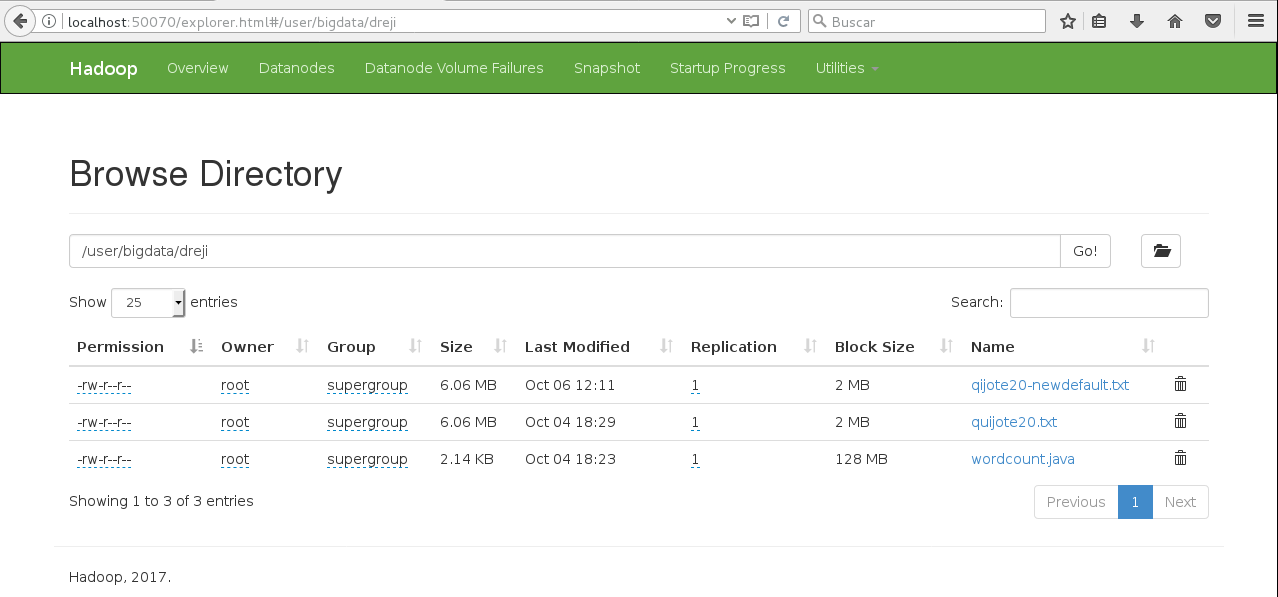
\includegraphics[scale=0.5]{figures/quijote20}
  \caption{Captura del explorador del HDFS de hadoop}
\end{figure}

Podemos ver cómo las dos versiones del \inline{quijote20.txt} subidas tienen tamaño de bloque de 2MB, mientras que cuando subimos un archivo antes de cambiar el valor de tamaño de bloques por defecto, este tenía 128MB de tamaño de bloque. Esto responde a los apartados 4.1, 4.2 y 4.3 del guión.


\newpage

\section{ Tutorial de Spark}

Seguimos el tutorial de spark y contestamos a las preguntas que se nos piden


\subsubsection*{ Pregunta TS1.1 ¿Cómo hacer para obtener una lista de los elementos al cuadrado?}

Bastará en este caso usar sobre el RDD la función map pasándole como parámetro la función  \inline{lambda x: x*x} que eleva el número al cuadrado. El código es este, con el resultado debajo:

\begin{minted}{python}
numeros = sc.parallelize([1,2,3,4,5,6,7,8,9,10])
cuadrados = numeros.map(lambda x : x*x)
print(cuadrados.collect())

[1, 4, 9, 16, 25, 36, 49, 64, 81, 100]
\end{minted}
\subsubsection*{ Pregunta TS1.2 ¿Cómo filtrar los impares? }

El código se nos entrega resuelto en este caso. Es bastante sencillo, si usamos sobre el RDD la función  \inline{filter} dándole como parámetro la función que calcula si cada elemento es impar, esto es, si su módulo 2 es 1 :  \inline{lambda x : x%2 == 1}, nos da todos los impares. El código completo es:

\begin{minted}{python}
rddi = numeros.filter (lambda e: e%2==1)
print (rddi.collect())

[1, 3, 5, 7, 9]
\end{minted}

\subsubsection*{ Pregunta TS1.3 ¿Tiene sentido esta operación? ¿Si se repite se obtiene siempre el mismo resultado?}

Nos encontramos con el siguiente código:
\begin{minted}{python}
#Tiene sentido esta operacion?
numeros = sc.parallelize([1,2,3,4,5])

print (numeros.reduce(lambda elem1,elem2: elem1-elem2))

\end{minted}

Esta operacion no tiene sentido, pues para hacer el reduce necesitamos que la operación sea conmutativa, es decir, que $a-b = b-a$, lo cual \textbf{NO} es cierto en todos los casos. Por eso además no producirá siempre los mismos resultados. Si ejecutamos en múltiples ocasiones veremos que los resultados no son los mismos siempre.

\subsubsection*{ Pregunta TS1.4 ¿Cómo lo ordenarías para que primero aparezcan los impares y luego los pares?}

Lo haremos para el caso general. Nos damos cuenta primero de que si el vector tiene $n$ posiciones y tratamos de tomar $m > n$ posiciones, Spark se quedará con todas las posibles. Por tanto, lo primero que hacemos es obtener un entero con el máximo de elementos

\begin{minted}{python}
numeros = sc.parallelize([3,2,1,4,5])

n = numeros.count()
\end{minted}

Por último, basta ahora tomar elementos ordenados especificando cuál es el criterio de orden. En este caso, queremos que los elementos pares sean los más grandes, por lo que debemos pasarle como argumento la función  \inline{lambda x: x%2 == 0}. De esta manera, escribiendo la línea siguiente, obtenemos el resultado.
\begin{minted}{python}
print(numeros.takeOrdered(n,lambda elem: elem%2== 0))

[3, 1, 5, 2, 4]
\end{minted}


\subsubsection*{ Pregunta TS1.5 ¿Cuántos elementos tiene cada rdd? ¿Cuál tiene más? }

Nos encontramos con el siguiente código

\begin{minted}{python}
lineas = sc.parallelize(['', 'a', 'a b', 'a b c'])

palabras_flat = lineas.flatMap(lambda elemento: elemento.split())
palabras_map = lineas.map(lambda elemento: elemento.split())

print (palabras_flat.collect())
print (palabras_map.collect())
\end{minted}
Cuya salida es:
\begin{minted}{python}
['a', 'a', 'b', 'a', 'b', 'c']
[[], ['a'], ['a', 'b'], ['a', 'b', 'c']]
\end{minted}
Para ver cuántos elementos tiene cada uno, podemos hacer 
\begin{minted}{python}
print(palabras_flat.count())
print(palabras_map.count())

6
4
\end{minted}

Claramente,  \inline{palabras_flat} tiene más. Esto ocurre porque en \inline{flatMap }cada elemento de entrada al que se le aplica la función \inline{lambda }puede tener como salida 0 o más (un vector) de elementos. Por tanto:
\begin{itemize}
\item Con \inline{flatMap }para cada elemento de \inline{lineas }obtenemos un vector que luego separaremos por elementos e ignoraremos los elementos que estén vacíos. Por ello, de 4 elementos iniciales pasamos a 6 que es el total de letras que tenemos en el RDD.
\item Con \inline{map }a cada uno de los vectores iniciales se le aplica la función indicada y se introduce \textbf{tal cual} en el RDD resultante, no se separan los elementos de los vectores obtenidos como ocurría en el caso anterior.
\end{itemize}

\subsubsection*{ Pregunta TS1.6 ¿De qué tipo son los elementos del rdd palabras\_map? ¿Por qué palabras\_map tiene el primer elemento vacío?}

Siguiendo la respuesta de la pregunta anterior, en \inline{palabras_map }los elementos obtenidos tras aplicar a cada elemento de  \inline{lineas }la función, son vectores, por lo que los elementos de \inline{palabras_map} son vectores.  Lo podemos ver en la salida del código

\begin{minted}{python}
print (palabras_map.collect())

[[], ['a'], ['a', 'b'], ['a', 'b', 'c']]
\end{minted}

Además, tiene el primer \textbf{elemento vacío} porque la función split aplicada sobre el elemento \inline{'' }devuelve un vector vacío pues no hay nada que separar.


\subsubsection*{ Pregunta TS1.7. Prueba la transformación distinct si lo aplicamos a cadenas.}

Para probarlo, realizamos el siguiente código en el que ponemos en un RDD ejemplos de prueba con las mismas palabras en mayúscula y minúscula, con espacios o signos de puntuación:

\begin{minted}{python}
test = sc.parallelize(["abcd", "abcd","dcba","abCd","a bcd","hola","HOLA","hola!","HoLa","ho la"])

dis = test.distinct()

print(dis.collect())
\end{minted}
La salida que obtenemos es:

\begin{minted}{python}
['abcd', 'abCd', 'a bcd', 'hola', 'hola!', 'dcba', 'HOLA', 'HoLa', 'ho la']
\end{minted}

Como podemos ver, teníamos un único ejemplo duplicado (el primero) que es el único que se ha eliminado. Esto nos indica que el comparador de elementos de los rdd comparan los strings *caracter a caracter*.

\subsubsection*{ Pregunta TS1.8 ¿Cómo se podría obtener la misma salida pero utilizando una sola transformación y sin realizar la unión?}


Se podría hacer que el filtro se quede con los elementos que empiecen por I o por E, haciendo el código del siguiente modo:

\begin{minted}{python}
log = sc.parallelize(['E: e21', 'I: i11', 'W: w12', 'I: i11', 'W: w13', 'E: e45'])

inferr = log.filter(lambda elem: elem[0] in ['I','E'])


print(inferr.collect())

'E: e21', 'I: i11', 'I: i11', 'E: e45']

\end{minted}
\subsubsection*{ Pregunta TS1.9 ¿Cómo explica el funcionamiento de las celdas anteriores?}

Comentamos una a una las celdas anteriores:

\begin{minted}{python}
numeros = sc.parallelize([1,2,3,4,5])

print (numeros.reduce(lambda elem1,elem2: elem2+elem1))
\end{minted}

Esta primera celda solo crea un RDD y luego hace la operación reduce, que combina los valores usando una función que le indicamos, en este caso la suma de los valores. Así, devolverá la suma de todos los valores ya que esta operación es conmutativa y asociativa.


\begin{minted}{python}
#Tiene sentido esta operacion?
numeros = sc.parallelize([1,2,3,4,5])

print (numeros.reduce(lambda elem1,elem2: elem1-elem2))
\end{minted}

Esta celda hace lo mismo que la anterior salvo que la operación que realiza es la resta. Como ya hemos visto en una pregunta anterior, esta operación no tiene sentido pues la resta no es una operación conmutativa por lo que el resultado no siempre será el mismo.

\begin{minted}{python}
palabras = sc.parallelize(['HOLA', 'Que', 'TAL', 'Bien'])

pal_minus = palabras.map(lambda elemento: elemento.lower())

print (pal_minus.reduce(lambda elem1,elem2: elem1+"-"+elem2))
#y esta tiene sentido esta operacion?
# Que pasa si ponemos elem2+"-"+elem1
\end{minted}

En esta celda se crea un RDD que tiene cadenas de caracteres, primero se pasan a minúsculas aplicándoles la funcion \inline{.lower }y luego se concatenan todas las palabras a un solo scring uniéndolas por guiones, obteniendo como salida:
\begin{minted}{bash}
hola-que-tal-bien
\end{minted}

Si cambiásemos el orden en elq ue se concatenan los elementos como se nos indica en el comentario, la salida cambia y las palabras se van uniendo en el orden inverso, debido a cómo se realiza la operación reduce. La salida es:
\begin{minted}{bash}
bien-tal-que-hola
\end{minted}

\begin{minted}{python}
r = sc.parallelize([('A', 1),('C', 4),('A', 1),('B', 1),('B', 4)])
rr = r.reduceByKey(lambda v1,v2:v1+v2)
print (rr.collect())
\end{minted}

En esta celda se crea un RDD que tiene como elementos Tuplas  \inline{(clave,valor)}. A continuación, usando \inline{reduceByKey }pasándole como argumento una función suma, lo que se hace es sumar los valores de las tuplas cuya clave sea la misma, obteniendo la salida esperada:
\begin{minted}{bash}
[('C', 4), ('A', 2), ('B', 5)]
\end{minted}

La última celda es la siguiente:
\begin{minted}{python}
r = sc.parallelize([('A', 1),('C', 4),('A', 1),('B', 1),('B', 4)])
rr1 = r.reduceByKey(lambda v1,v2:v1+v2)
print (rr1.collect())
rr2 = rr1.reduceByKey(lambda v1,v2:v1)
print (rr2.collect())
\end{minted}

De nuevo, se crea un RDD cuyos elementos son tuplas  \inline{(clave,valor)} , primero se realiza lo mismo que en la celda anterior, y luego se vuelve a aplicar sobre el RDD obtenido la función \inline{reduceByKey }esta vez pasándole como función simplemente mantenerla clave que tiene. Sin embargo, esto no parece producir ningún efecto sobre el RDD, pues cuando se realiza la operación  \inline{collect }para ver los elementos del mismo, la salida es la misma que se produce en la celda anterior.

Como \textbf{conclusión} a esta pregunta, podemos decir que es importante cómo se aplica la función \inline{reduce }sobre los RDD y que hay que tener cuidado con las operaciones que indicamos a esta función pues podrían no producir los resultados que se desean. 

\subsubsection*{ Pregunta  \inline{groupByKey}}

Dada la siguiente celda
\begin{minted}{python}
r = sc.parallelize([('A', 1),('C', 2),('A', 3),('B', 4),('B', 5)])
rr = r.groupByKey()
res= rr.collect()

print(rr.collect())


# Que operacion realizar al RDD rr para que la operacion sea como un reduceByKey
\end{minted}

Lo priemro que vemos es que la operación \inline{rr.collect }devuelve una lista con tuplas  \inline{(clave, pyspark Result Iterable)}. Estos iterables debemos pasarlos primero a una lista, y luego realizar sobre ellos la operación que quisiésemos hacer con el  \inline{reduceByKey}. Vemos que los pasamos a una lista utilizando \inline{mapValues(list) }que convierte los valores a un tipo:

\begin{minted}{python}
rrf = rr.mapValues(list).collect()
print(rrf)

[('C', [2]), ('A', [1, 3]), ('B', [4, 5])]
\end{minted}

Y, a continuación, podemos realizar la operación que haríamos con el reduce. Por ejemplo, si queremos hacer la suma de los vectores utilizando \inline{map }podríamos hacer todo en una linea de la siguiente manera:
\begin{minted}{python}
rrf = rr.mapValues(list).map(lambda x : (x[0],sum(x[1])))
print(rrf.collect())

[('C', 2), ('A', 4), ('B', 9)]
\end{minted}

Ahora, se nos pide simular el \inline{groupByKey }usando \inline{reduceByKey }y  \inline{map}. Para ello, usando \inline{reduceByKey }podemos obtener las listas que obtendríamos tras aplicar el \inline{mapValues(list) }que hemos obtenido anteriormente.
\begin{minted}{python}
simul_group = r.reduceByKey(lambda v1,v2: [v1,v2])
print(simul_group.collect())

[('C', 2), ('A', [1, 3]), ('B', [4, 5])]
\end{minted}

\subsubsection*{ Pregunta sobre  \inline{join}}

\begin{minted}{python}
rdd1 = sc.parallelize([('A',1),('B',2),('C',3)])
rdd2 = sc.parallelize([('A',4),('B',5),('C',6)])

rddjoin = rdd1.join(rdd2)
\end{minted}

El resultado de esto es 
\begin{minted}{bash}
[('A', (1, 4)), ('B', (2, 5)), ('C', (3, 6))]
\end{minted}

Es decir, un nuevo RDD en el que los valores son tuplas con los valores que hay en cada uno de los RDD. Se nos pide que, dado ese código, cambiemos las claves de los dos RDDs iniciales para ver qué RDD se crea finalmente. Si lo hacemos, cambiando por ejemplo los RDD del siguiente modo:
\begin{minted}{python}
rdd1 = sc.parallelize([('A',1),('B',2),('D',3)])
rdd2 = sc.parallelize([('A',4),('B',5),('E',6)])

rddjoin = rdd1.join(rdd2)
\end{minted}
El resultado obtenido es el siguiente:
\begin{minted}{bash}
[('A', (1, 4)), ('B', (2, 5))]
\end{minted}
Es decir, que el \inline{join }está haciendo la unión de los elementos cuyas claves están en la intersección del conjunto de claves. Como \inline{D }y \inline{E }no están en ambos RDD, no están en la intersección del conjunto de claves y por tanto no se obtienen en el RDD final.

\subsubsection*{ Tipos de Join }

Se nos pregunta que qué ocurre cuando sustituimos \inline{join }por \inline{leftOuter/rightOuter/fullOuter }join. El resultado es que estos tipos de \inline{join }crean elementos en el nuevo RDD aunque sus claves no estén en ambos RDD iniciales. En concreto:
\begin{itemize}
\item  \inline{leftOuter }añade al nuevo RDD también las tuplas  \inline{(clave,valor)} cuya clave esté en el \inline{RDD }sobre el que se llama la función, pero no estén en el RDD que se pasa como parámetro. Se añade un \inline{None }en la tupla conjunta del RDD final:
\begin{minted}{python}
rdd1 = sc.parallelize([('A',1),('B',2),('C',3)])
rdd2 = sc.parallelize([('A',4),('A',5),('B',6),('D',7)])
rddjoin = rdd1.leftOuterJoin(rdd2)

[('A', (1, 4)), ('A', (1, 5)), ('B', (2, 6)), ('C', (3, None))]
\end{minted}

\item  \inline{rightOuter} hace lo mismo que el anterior pero en el sentido opuesto, es decir, usando el segundo RDD.
\item  \inline{fullOuter} combina los dos anteriores.

\end{itemize}

\subsubsection*{ Pregunta TS1.10 Borra la salida y cambia las particiones en parallelize. ¿ Qué sucede ?}

Lo que ocurre si ponemos 10 particiones es lo siguiente (borrando anteriormente el contenido del directorio donde tenemos la salida):
\begin{minted}{python}
numeros = sc.parallelize(range(0,1000),10)
numeros.saveAsTextFile('salida')

%ls -la salida/*



-rw-r--r-- 1 root root 290 Oct  4 10:42 salida/part-00000
-rw-r--r-- 1 root root 400 Oct  4 10:42 salida/part-00001
-rw-r--r-- 1 root root 400 Oct  4 10:42 salida/part-00002
-rw-r--r-- 1 root root 400 Oct  4 10:42 salida/part-00003
-rw-r--r-- 1 root root 400 Oct  4 10:42 salida/part-00004
-rw-r--r-- 1 root root 400 Oct  4 10:42 salida/part-00005
-rw-r--r-- 1 root root 400 Oct  4 10:42 salida/part-00006
-rw-r--r-- 1 root root 400 Oct  4 10:42 salida/part-00007
-rw-r--r-- 1 root root 400 Oct  4 10:42 salida/part-00008
-rw-r--r-- 1 root root 400 Oct  4 10:42 salida/part-00009
-rw-r--r-- 1 root root   0 Oct  4 10:42 salida/_SUCCESS
\end{minted}

Como se podía esperar, se crea un archivo para cada una de las particiones de salida, según el número de particiones que le hayamos indicado.

\subsection{Procesamiento El Quijote}

\subsubsection*{ Pregunta TS2.1 Explica la utilidad de cada transformación y detalle para cada una de ellas si cambia el número de elementos en el RDD resultante. Es decir si el RDD de partida tiene N elementos, y el de salida M elementos, indica si N>M, N=M o N<M.}

Dado el siguiente código:
\begin{minted}{python}
charsPerLine = quijote.map(lambda s: len(s))
allWords = quijote.flatMap(lambda s: s.split())
allWordsNoArticles = allWords.filter(lambda a: a.lower() not in ["el", "la"])
allWordsUnique = allWords.map(lambda s: s.lower()).distinct()
sampleWords = allWords.sample(withReplacement=True, fraction=0.2, seed=666)
weirdSampling = sampleWords.union(allWordsNoArticles.sample(False, fraction=0.3))
\end{minted}
Se nos pide indicar qué hace cada una de las transformaciones. Procedemos línea a línea:

\begin{enumerate}
\item  \inline{charsPerLine = quijote.map(lambda s: len(s)) }esta línea obtiene un nuevo RDD en el que se cambian las líneas del quijote por la longitud de cada línea. No se modifica el número de elementos, se tiene $N = M$.

\item  \inline{allWords = quijote.flatMap(lambda s: s.split()) } obtiene un nuevo RDD en el que se separa cada uno de los strings iniciales en cada una de sus palabras y luego cada palabra se convierte en un elemento del RDD. Por tanto, el RDD de salida tiene muchos más elementos que el de entrada, podemos decir que $M >> N$.

\item  \inline{allWordsNoArticles = allWords.filter(lambda a: a.lower() not in ["el", "la"])} se toma el RDD de las palabras y se pasa un filtro que elimina todos los artículos *el* y *la* (sin distinción de mayúsculas/minúsculas) del documento. Al eliminar elementos, el número de elementos en la salida será menor que en la entrada por lo que $M < N$.

\item  \inline{allWordsUnique = allWords.map(lambda s: s.lower()).distinct() }se crea un RDD que tiene un elemento por cada palabra distinta (sin distinción mayúsculas/minúsculas) que haya en el RDD  \inline{allWords}. De nuevo, se eliminan elementos repetidos por lo que el número de elementos en la salida será menor que en la entrada, $M < N$.

\item  \inline{sampleWords = allWords.sample(withReplacement=True, fraction=0.2, seed=666)} se extrae aleatoriamente con reemplazamiento un $20\%$ de las palabras que hay en \inline{allWords }para crear un nuevo RDD. Por supuesto, se tendrá que $M = 0.2 N$ ($M < N$).

\item  \inline{weirdSampling = sampleWords.union(allWordsNoArticles.sample(False, fraction=0.3))} priemro extrae sin reemplazamiento un $30\%$ de elementos que tenemos en el RDD que no tiene artículos (en este caso, tendríamos $M < N$ pues reducimos elementos) y a continuación une estos elementos extraídos al RDD que tiene una muestra del $20\%$ que hemos obtenido en el paso anterior. En esta unión aumenta el tamaño del RDD por lo que en este paso $M > N$.

\end{enumerate}
Ahora, explicamos las funciones en general, su utilidad y si cambia el número de elementos del RDD resultante:

\begin{itemize}

\item  \inline{map }sirve para realizar una transformación sobre el RDD pasándole como parámetro una función. El número de elementos final del RDD es el mismo, pues a cada elemento se le aplica una función pero sigue siendo un elemento, no se elimina ninguno, por lo que $M=N$.

\item  \inline{flatmap }realiza una transformación y, a continuación, si tenemos vectores como puntos, hace que cada elemento de los vectores sea un punto del nuevo RDD, por lo que en este caso el número se mantiene (si cada vector de salida tiene dimensión 1), o aumenta, por lo que $M \geq N$.

\item  \inline{filter }selecciona un conjunto de elementos según una función que da una condición implícita. Todos los elementos pueden cumplir esa condición o solo un subconjunto de ellos, por lo que $M \leq N$.

\item  \inline{distinct }toma los elementos del RDD que sean únicos (diferentes a todos los demás). Todos podrían ser diferentes o podría haber elementos iguales, por lo que $M \leq N$.

\item  \inline{sample }toma una muestra del tamaño indicado. En este caso, el RDD no se modifica solo que se toman ejemplos del mismo, por lo que podemos decir que el tamaño del RDD se mantiene, $M=N$.

\item  \inline{union }une dos RDDs en uno

\end{itemize}


\end{document}
